\section{Proposed Graphics}

The goal of this visualization project is to provide a cross-section of American life and well-being through a juxtaposition of citizens in two very different years, 1968 and 2014, at time of death.



\subsection{Cause of Death}

Cause of death can offer clues as to how a person lived; on a mass scale, cause of death statistics can reflect the overall health of a nation.

\begin{enumerate}
\item \textit{Cause of Death by Location}\\
A map is proposed that highlights the leading cause of death by US state, with an animated function switching between 1968 and 2014.

\begin{figure}[H]
\centering
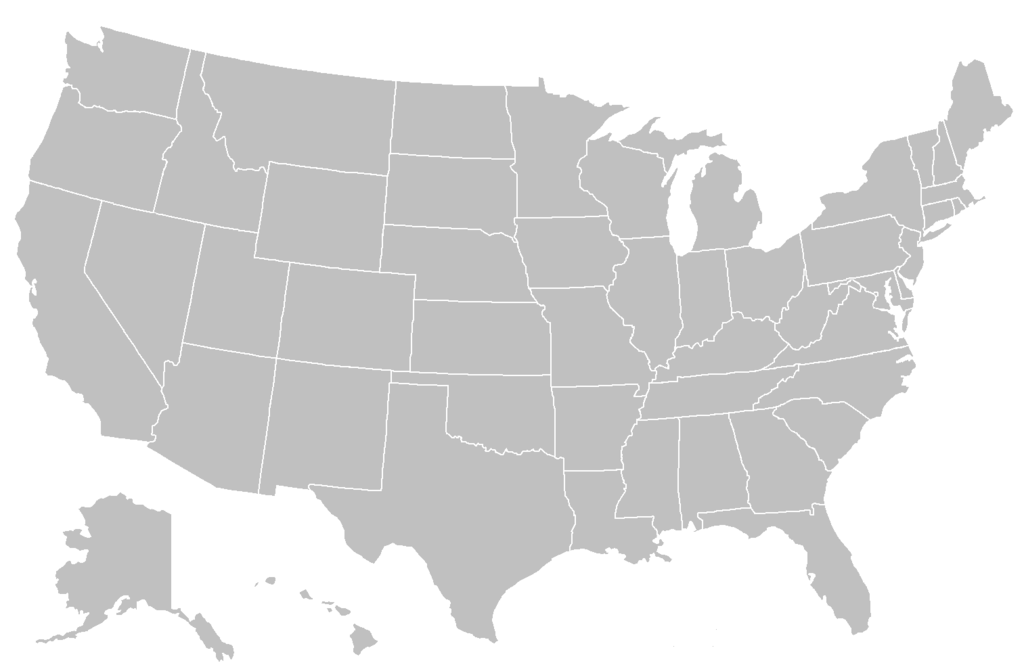
\includegraphics[width=0.5\linewidth]{usa_blank.png}
\caption{A blank map of states similar to the one that would be color-coded with cause of death in this proposed visualization.}
\end{figure}

\item \textit{Cause of Death vs. Age of Death}\\
A plot is proposed that identifies the three leading causes of death for each age group, grouped together in five-year intervals, in hopes of identifying the \textit{risk periods}: specific ages at which a person may be threatened by a specific disease/factor.

\item \textit{Cause of Death by Race}\\
What are the leading killers of people of different ethnic backgrounds? A plot is proposed to display the handful of leading causes of death for each race identified in the dataset.

\item \textit{Cause of Death by Gender}\\
Are there diseases that primarily target on sex over the other? A plot is proposed to show the discrepancies between deaths of citizens of different genders from the same ailment.
\end{enumerate}



\subsection{Age of Death}

Age at time of death is a key statistic for the evaluation of the health of a populace. Life expectancy statistics are extremely widespread, but do not offer the full picture. This section of visualizations aims to clear up some of the ambiguity surrounding that particular statistic.

\begin{enumerate}
\item \textit{Age of Death by Race}\\
Is there a difference in life expectancy for different ethnic groups? A simple bar plot is proposed to show the average life expectancy based on deaths in 1968 and 2014 for the different groups identified in the CDC dataset.

\item \textit{Age of Death vs. Gender}\\
Most of us know that women are expected to live longer than men; if this is indeed true, what do the death rates by age look like for the two different genders? Is there a particular period in life in which many men die but many women live through?

\item \textit{Age of Death by Location}\\
Which states die young? Are there states that are substantially more healthy (in that they live longer) than others? How do the trends identified in the \textit{race} and \textit{gender} plots hold up when grouped by state boundaries?

\end{enumerate}

Additional plots may be included as familiarity with the dataset and its offerings increases.


\section{Presentation and Technologies}

As an experienced web developer the findings from this project will be organized an presented as a single, interactive web page.

The forecasted technologies for presentation include \texttt{HTML/CSS} (of course), \texttt{JavaScript}, \texttt{plotly} (either \texttt{js} or \texttt{R}), and likely \texttt{ggplot2}.

For data processing before visualization, I will write processing scripts in the functional programming language \texttt{OCaml}. This language is quite powerful and is well-suited for sifting and sorting through large datasets such as those provided by the CDC.

